\documentclass[10pt,twocolumn,letterpaper]{article}

\usepackage{cvpr}
\usepackage{times}
\usepackage{epsfig}
\usepackage{graphicx}
\usepackage{amsmath}
\usepackage{amssymb}

\usepackage{tikz}
\usepackage{pgfplots}
\usepackage{siunitx} % Required for alignment
\usepackage{booktabs} % For prettier tables
\usepackage{multirow}

\usepackage[font=small,labelfont=bf]{caption} % Required for specifying captions to tables and figures
\usepackage[subrefformat=parens]{subcaption}

% Include other packages here, before hyperref.

% If you comment hyperref and then uncomment it, you should delete
% egpaper.aux before re-running latex.  (Or just hit 'q' on the first latex
% run, let it finish, and you should be clear).
\usepackage[breaklinks=true,bookmarks=false]{hyperref}



\cvprfinalcopy % *** Uncomment this line for the final submission

\def\cvprPaperID{****} % *** Enter the CVPR Paper ID here
\def\httilde{\mbox{\tt\raisebox{-.5ex}{\symbol{126}}}}

% Pages are numbered in submission mode, and unnumbered in camera-ready
%\ifcvprfinal\pagestyle{empty}\fi
\setcounter{page}{1}
\begin{document}

%%%%%%%%% TITLE
\title{Fine-Grailed Classification Applied to Foliar Diseases in Apple Trees}

\author{Luca Rettenberger\\
Ravensburg-Weingarten \\ 
University of Applied Sciences \\
{\tt\small lr-192176@rwu.de}
}

\maketitle
%\thispagestyle{empty}

%%%%%%%%% ABSTRACT
\begin{abstract}
In this work we discuss the problem of solving a multiclass classification problem in which one class is not only rare, but a composition of other classes as well. Precisely we present our solution to the Plant Pathology challenge on Kaggle: \url{https://www.kaggle.com/c/plant-pathology-2020-fgvc7/}. Our solution uses a composition of the most state-of-the-art deep neural networks, which focus on being both fast and accurate.  In addition to that an ancillary deep network is trained, which specifically deals with the rare class. To support this additional network an sophisticated method for upsampling the rare class is used. This network is then braided into the composition of deep neural networks to form an architecture which is able to deal with the rare class while still classifying the other classes correctly. We achieve a score of             $\ 96.6\%$,  on the public leaderboard which is in the top $41\%$ of all competitors.
\end{abstract}

\section{Introduction}
If one wants to prevent an outbreak of disease in an apple orchard one either has to consult (or be) an expert for plant diseases, who are unfortunately rare and most of the time overbooked \cite{judd2017development, thapa2020plant}. Experts are needed because detecting and classifying diseases in an apple orchard is very hard and requires a lot of training. Without expertise it is not possible to distinguish between different diseases or evaluate how serious a situation is \cite{thapa2020plant}. But unnoticed diseases can lead to cosmetic unappealing apples and even to ones which are so diseased that they are unsuitable for sale \cite{sutton2014compendium}. This will lead to high economic losses and hence one needs to react fast if there is an outbreak of disease. Many experts in pant pathology use a combination of visual features found on the leafs of apple trees and automatic evaluation tools \cite{barbedo2014automatic}. However are such evaluation tools prune to human error because they need human intervention and are far from automatic  \cite{barbedo2014automatic}. Additionally to that are those tools often very complex and difficult to use  \cite{barbedo2014automatic}.

Both human experts and evaluation tools heavily evaluate visual indicators for detecting diseases, so to try to detect diseases solely on images feels natural. But visual indicators for foliar diseases range greatly depending on leaf color, ambient temperature, time of the day, age of the considered apple tree and a whole range of more variables \cite{dai2019high, thapa2020plant}. Because of that is the result sometimes unsatisfactory even if the consulted expert uses additional software and produces no errors \cite{thapa2020plant}. If it was possible to detect foliar diseases only with images, one could prevent disease outbreaks on apple orchards equipped only with a camera. Such a classification would be much faster and cheaper than consulting an expert on plant pathology. Some solutions to plant pathology have emerged in recent time which only rely on computer vision. But most of the solutions do not hold up to the expectation of classifying leafs while being on the apple orchard. Most existing solutions assume that the leafs are evaluated in an laboratory environment and hence to not deal with external influences like different backgrounds, different lighting conditions or other factors which come into play if the leafs should be classified on the apple orchard \cite{barbedo2014automatic, mohanty2016using, liu2018identification, dubey2016apple}.

Since this problem is unsolved Thapa et al. \cite{thapa2020plant} created an annotated dataset and started a Kaggle challenge (\url{https://www.kaggle.com/tarunpaparaju/plant-pathology-2020-eda-models}) to solve the problem of classifying leafs in an natural environment to be used on the go while walking through a apple orchard. This work tries to solve this problem with the provided dataset.
\section{Dataset}
The dataset is provided by the Plant Pathology and Plant-Microbe Biology Section of the Cornell University  \cite{thapa2020plant}. The dataset consists of images of leafs from apple trees under multiple health conditions. The images were taken from different angles, various illumination conditions  and several  different times of day. The dataset was generated directly from apple orchards. For more details see \cite{thapa2020plant}. 

The dataset consists of four disjoint classes, so every sample belongs to only one class. The classes are: \textit{Healthy}, \textit{Rust}, \textit{Scab} and \textit{Multiple diseases}. Every sample is an image of a leaf which belongs to one of the classes. There are $3642$ samples in total. $3619$ samples are of size $2048 \times 1365$. $23$ samples have flipped dimensions of $1365 \times 2048$. The samples are split into train images and validation images. There are $1821$ images in both categories (so it is a split in two halves). The labels for the train images are given. The validation images are unlabeled however, since they are used as performance evaluation in the Kaggle challenge. Figure \ref{exampleSamples} shows and example of every class.

\begin{figure*}[htb]
\begin{center}
\begin{subfigure}[b]{0.246\linewidth}
\centering
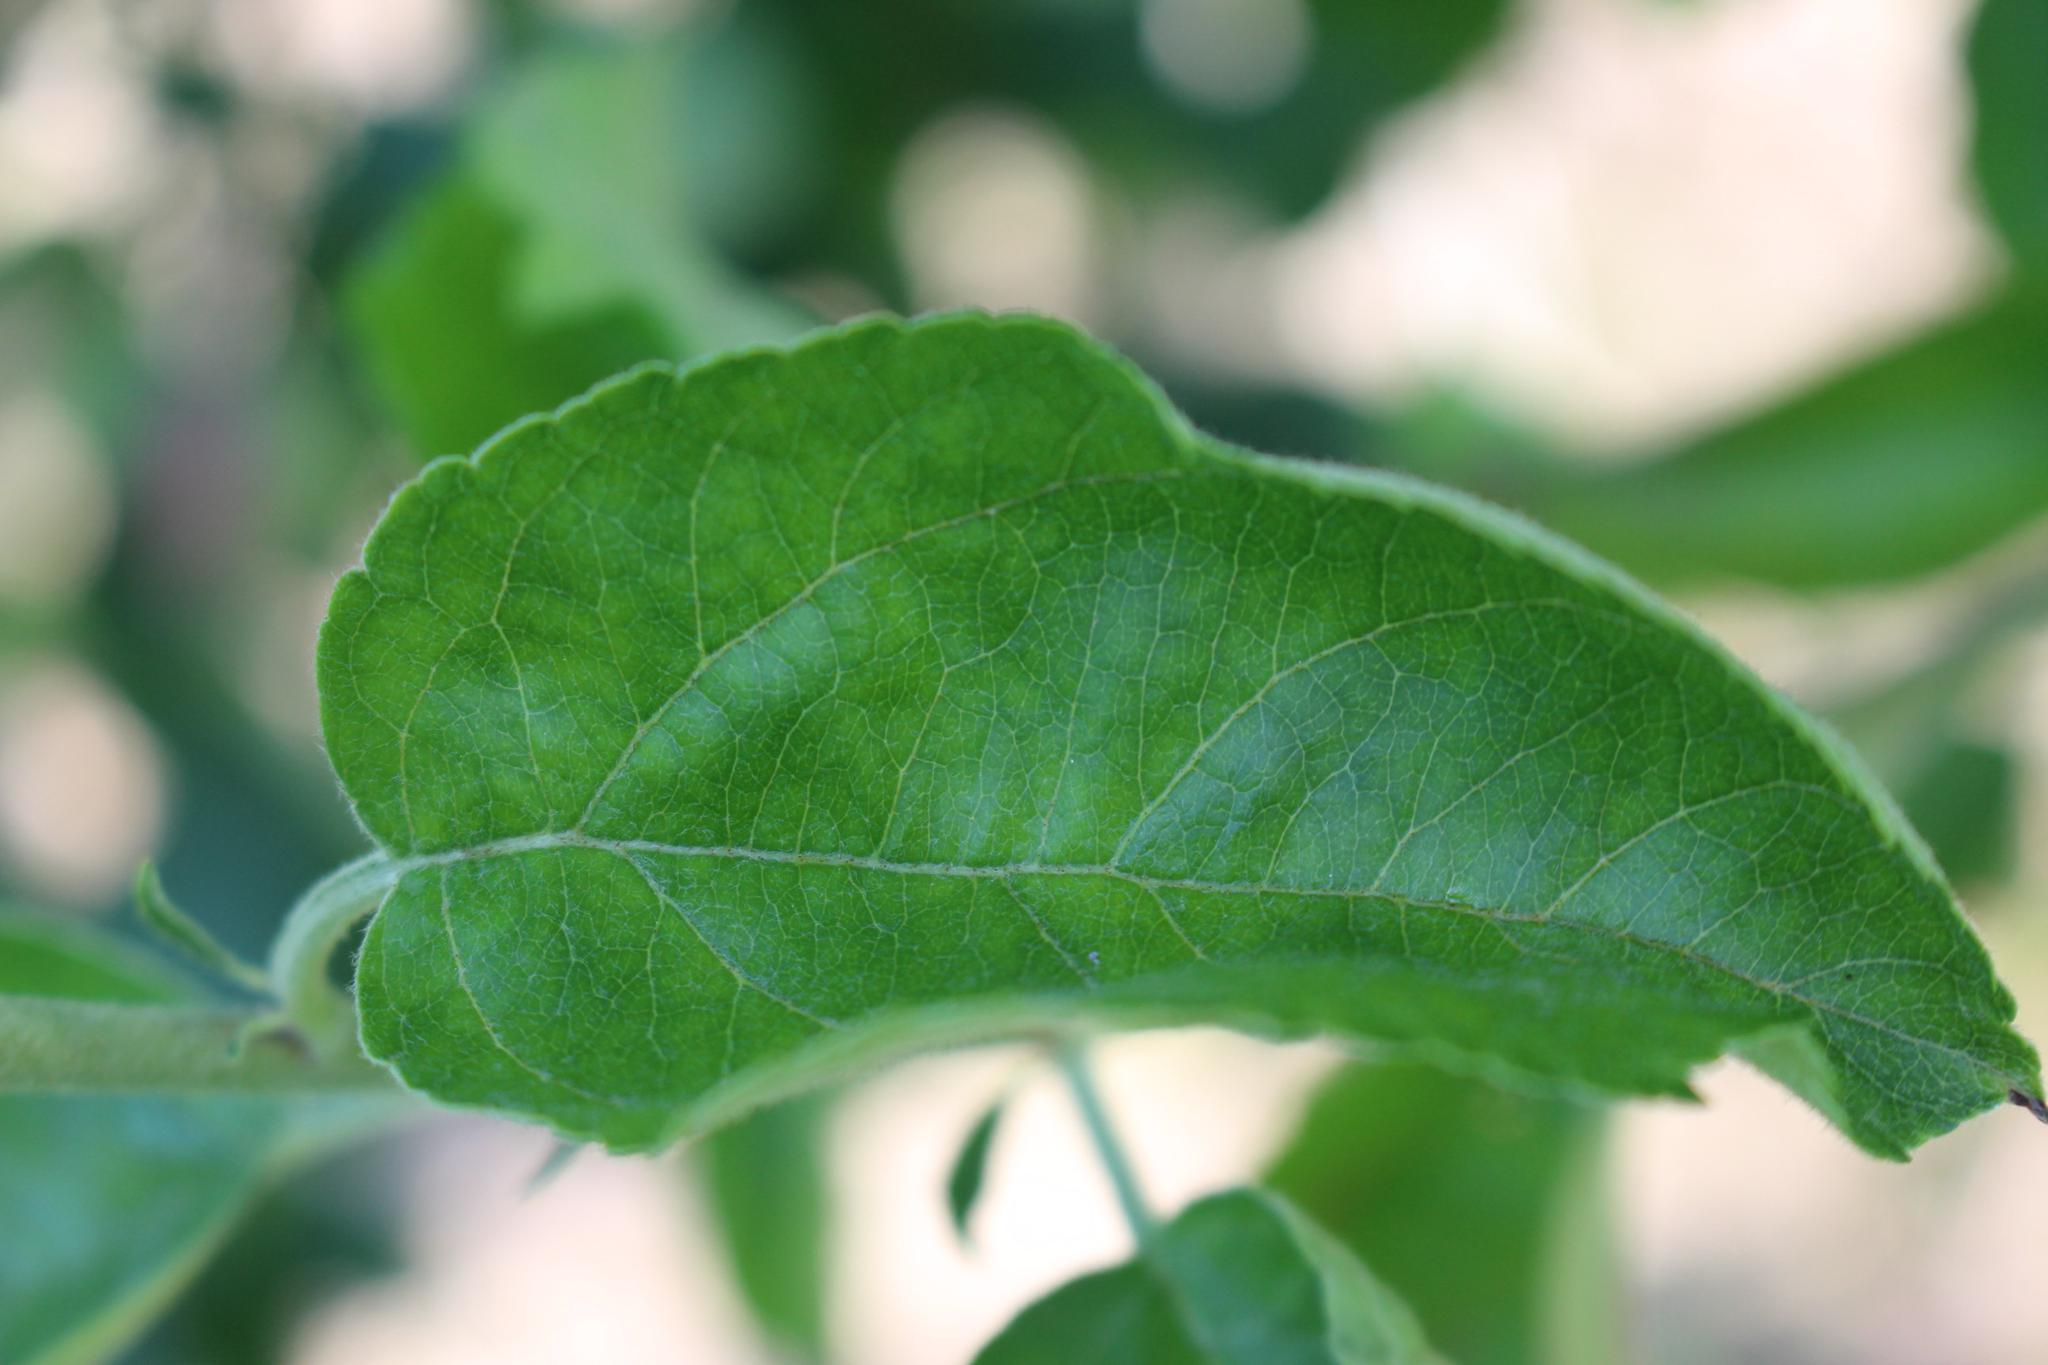
\includegraphics[width=\linewidth]{images/healthy.jpg}
\caption{Healthy Sample}\label{healthyFig}
\end{subfigure}
\begin{subfigure}[b]{0.246\linewidth}
\centering
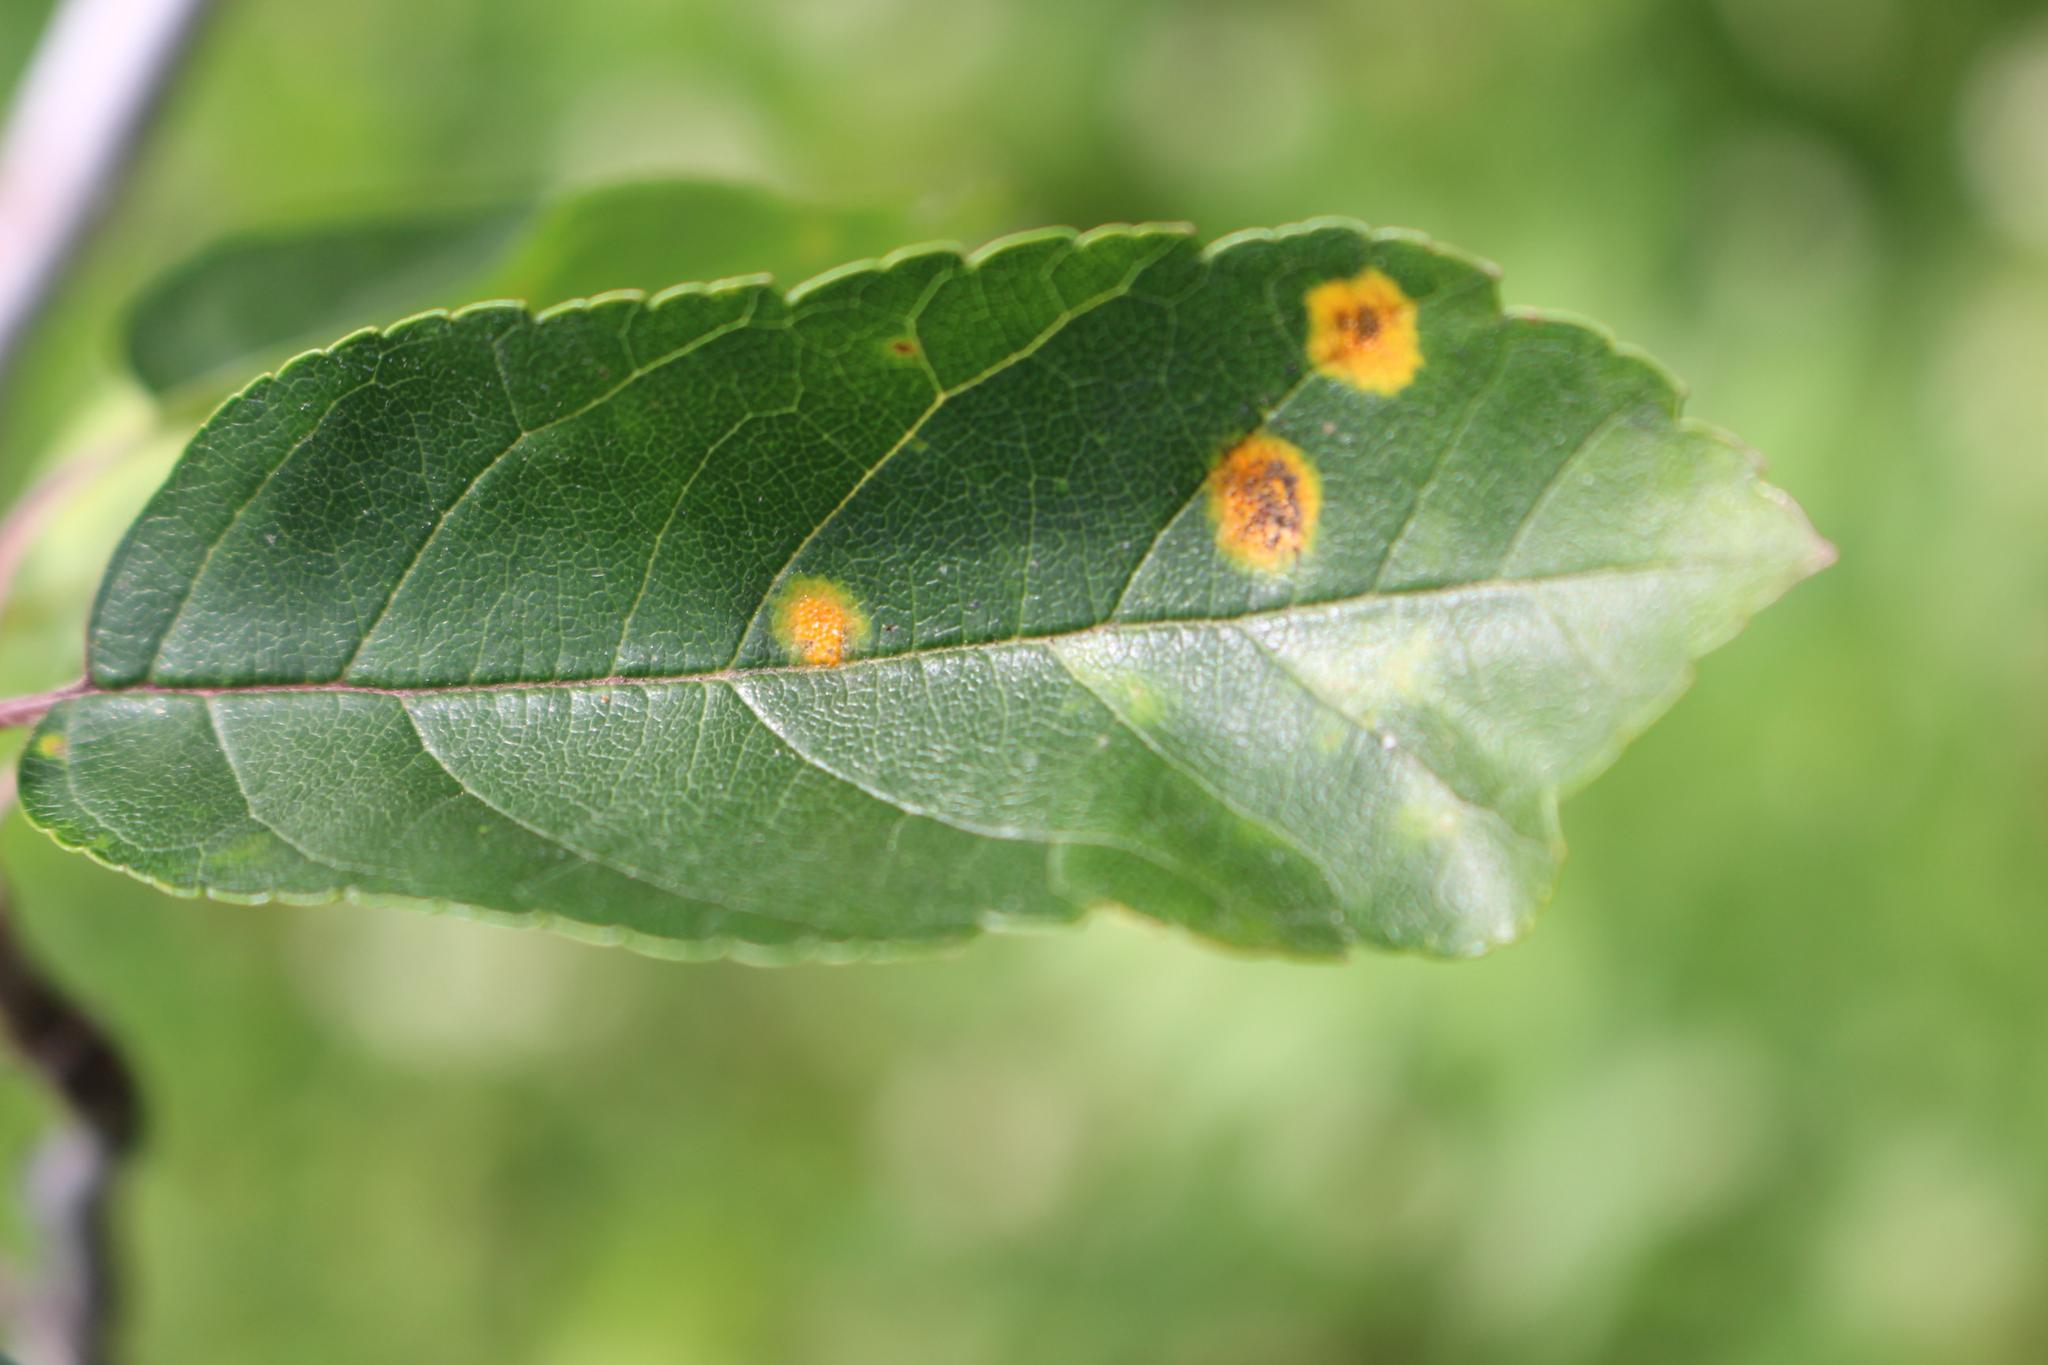
\includegraphics[width=\linewidth]{images/rust.jpg}
\caption{Rust Sample}\label{rustFig}
\end{subfigure}
\begin{subfigure}[b]{0.246\linewidth}
\centering
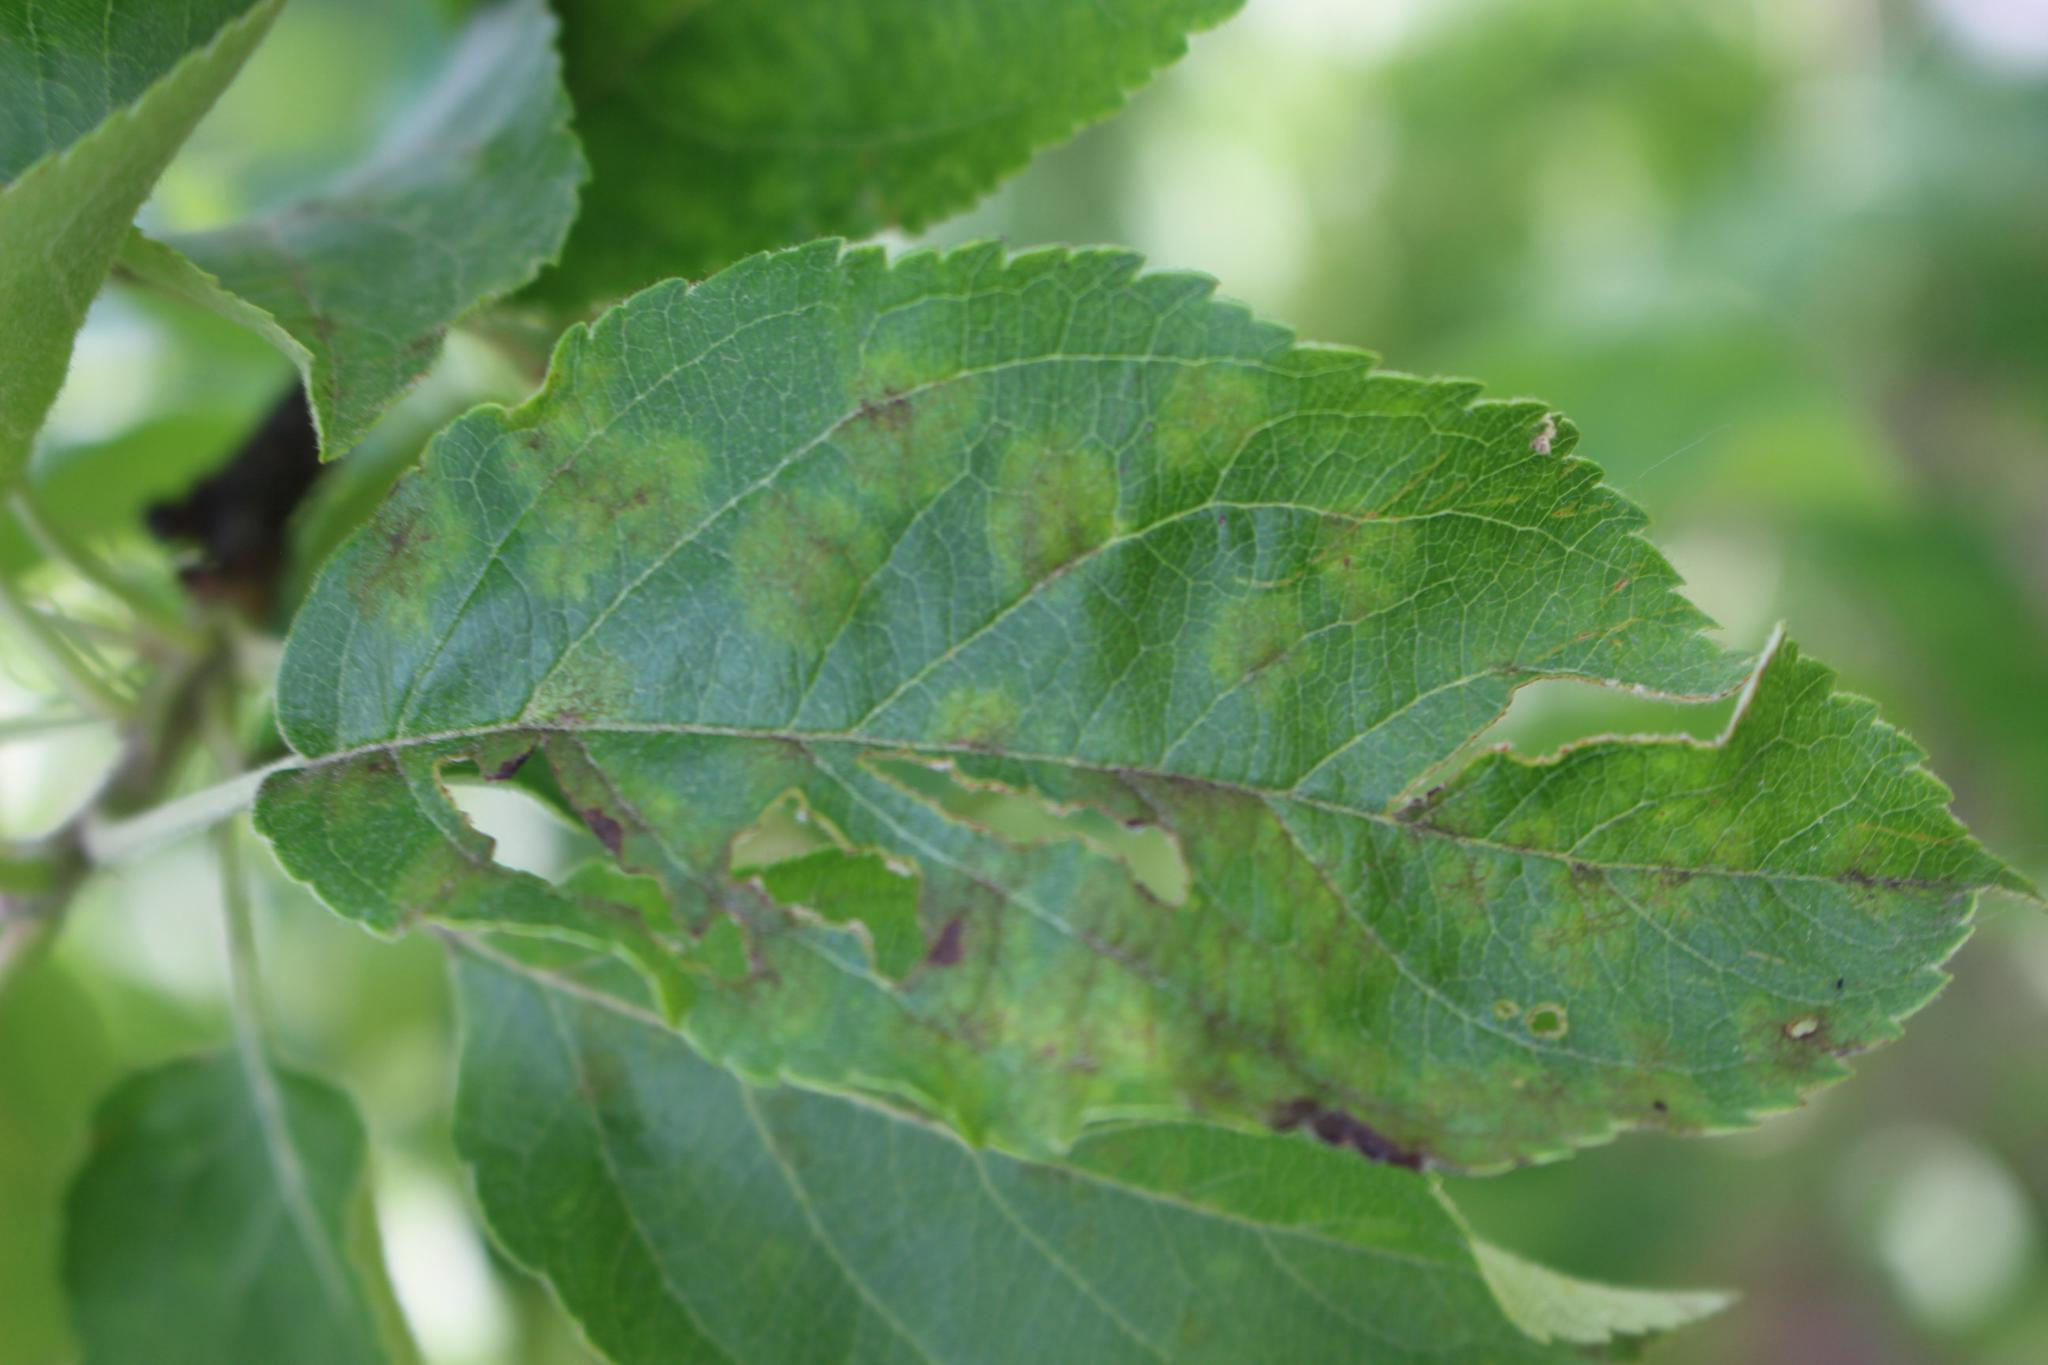
\includegraphics[width=\linewidth]{images/scab.jpg}
\caption{Scab Sample}\label{scabFig}
\end{subfigure}
\begin{subfigure}[b]{0.246\linewidth}
\centering
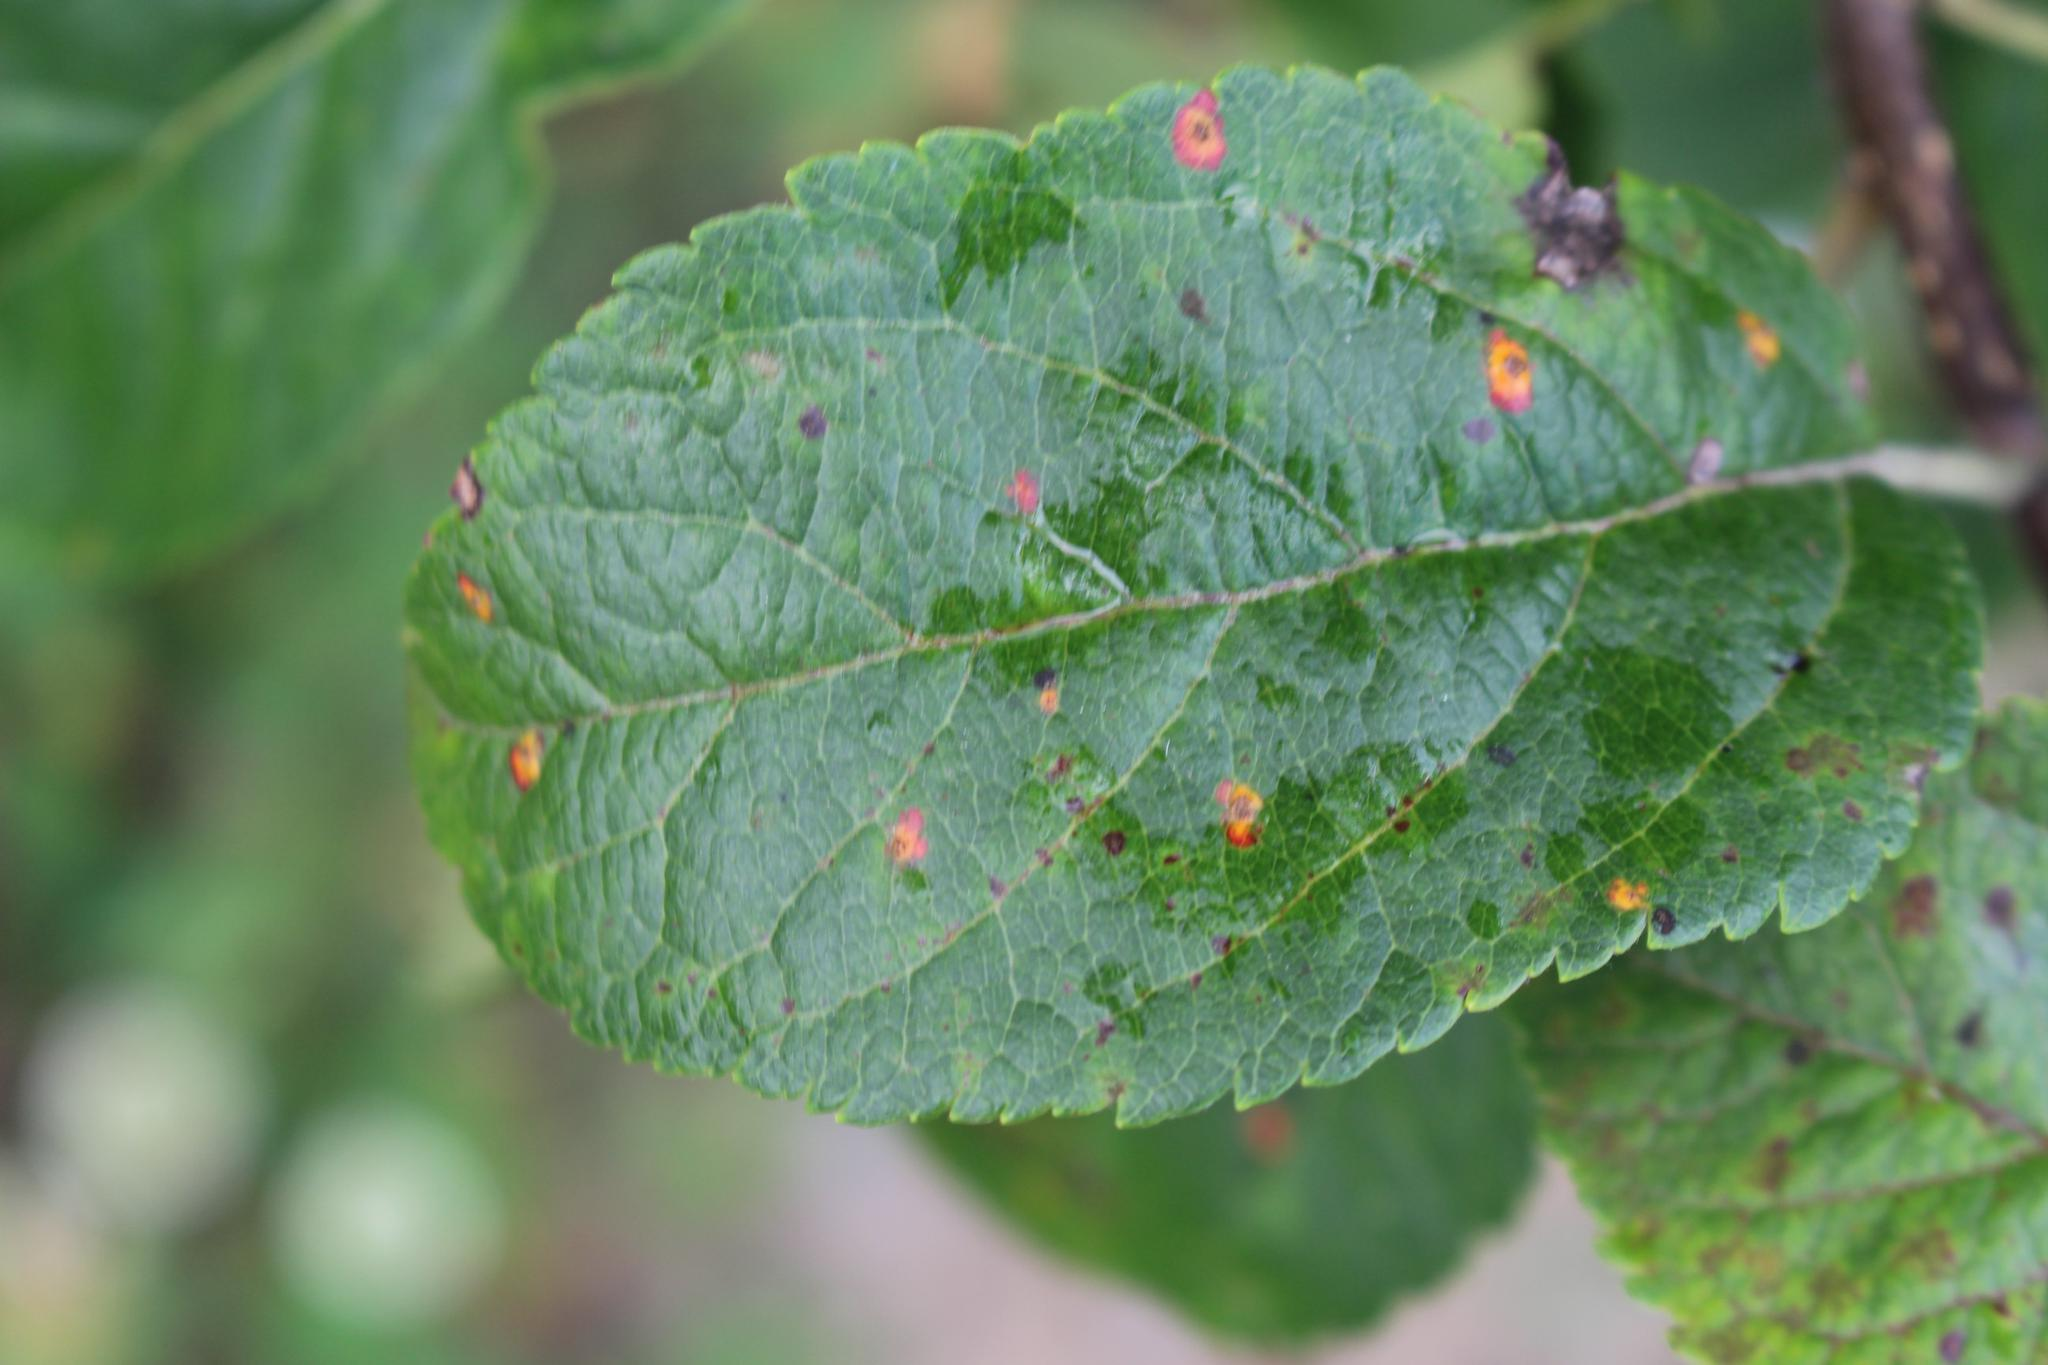
\includegraphics[width=\linewidth]{images/mult.jpg}
\caption{Multiple Diseases Sample}\label{multFig}
\end{subfigure}\hfill
\end{center}
   \caption{Examples of samples from all classes of the Plant Pathology Dataset. }
\label{exampleSamples}
\end{figure*}

\begin{table}[h!]
  \begin{center}
    \begin{tabular}{l|S|r}
      \toprule % <-- Toprule here
       \multirow{2}{*}{\textbf{Class}} & \multicolumn{2}{c}{\textbf{Frequency}}\\
       & \textbf{Absolute} & \textbf{Relative}\\
      \midrule % <-- Midrule here
      \textbf{Healthy} & 516& 28.34\%\\
      \textbf{Rust} & 622& 34.16\%\\
      \textbf{Scab} & 592 & 32.51\%\\
      \textbf{Multiple Diseases} & 91 & 5.00\%\\
      \bottomrule % <-- Bottomrule here
    \end{tabular}
     \caption{Class distribution of the Train Images.}
    \label{tab:frequencies}
  \end{center}
\end{table}

Since only the classes of the $1821$ training images are given merely they can be observed. The class distribution of the dataset is highly imbalanced. While the classes \textit{Healthy}, \textit{Rust} and \textit{Scab} are fairly balanced there is a lack of images of the \textit{Multiple diseases} class. For details see Table \ref{tab:frequencies}.
\section{Methods}
% How did i solve the problem?
The images of this dataset are all within the same class of "leafs" and hence it is not possible to rely on the high variance of different classes (e.g. differentiating between cats and dogs). The focus needs to be set on the fine grailed characteristics of the different classes. This problem is called fine-grained image classification \cite{akata2015evaluation}. This is especially difficult since the \textit{Multiple Diseases} class may contain properties contained in the \textit{Rust} and/or \textit{Scab} classes as well. One additional challenge is that the \textit{Multiple Diseases}  class is underrepresented and hence cannot be learned as easy as the other classes.  The main challenges of classifying the different leaf conditions are therefore:
\begin{itemize}  
	\setlength\itemsep{0.1em} 
  	\item Learn the fine-grailed features of the different leaf conditions.
	\item Compensate the few samples of the \textit{Multiple Diseases}  class.
\end{itemize}
Firstly some necessary preprocessing steps and image augmentation techniques are presented in section \ref{augmentation} to prepare the data for training, enrich the dataset and make it less prone to overfitting. Secondly the general problem of classifying the different leaf types is tackled in section \ref{ensemble}. After that, in section \ref{outlier_detection}, an additional technique is introduced which focuses on the rare \textit{Multiple Diseases} class. Finally, in section \ref{combined}, are the two methods of section \ref{ensemble} and section \ref{outlier_detection} combined to form a architecture which deals with the proposed problem in a composed way.
\subsection{Preprocessing and Image Augmentation} \label{augmentation}
The train images are once more split into a train- and test-data. 90\% (1639 images) of the images are used for training and 10\% (182 images) for testing. The datasets are referred to as "train-dataset" and "test-dataset" respectively. 

Even simple image augmentation has shown to have a great impact on the performance on deep neural networks \cite{perez2017effectiveness, simard2003best}. Other approaches to leaf classification usually use affine transformations, simple image rotations and perspective transformations \cite{sladojevic2016deep, wick2017leaf}. In this work the augmentation techniques are also mostly simple affine transformations. The augmentations are namely:
\begin{itemize}
	\setlength\itemsep{0.1em} 
  	\item Horizontal Flips.
	\item Vertical Flips.
	\item Rotations within a range of 10 degrees in both directions.
	\item Horizontal shifts in the range of 0\%-10\% of the total image width in both directions.
	\item Vertical shifts in the range of 0\%-10\% of the total image height in both directions.
	\item Zooms in the range of 90\%-110\% (so zooming 10\% in or out).
	\item Shearing transformations within a range of 10 degrees (counter-clockwise).
	\item Darken the image within a range of 50\% of the original brightness value.
	\item Brighten the image within a range of 50\% of the original brightness value.
	\item Box blur with a kernel size of $(5\times 5)$ to blur the image. \footnote{For more information about box blur see: \cite{wiki:blur}.}.
\end{itemize}
The augmentations are applied randomly when training data is sampled. The test-dataset is not augmented. If empty parts arise in the course of augmentation they are filled by duplicating the nearest pixels until the empty space is filled. All images are normalized by scaling the pixel values to the range of 0-1 ($1/255$). All images are scaled to a size of $(299 \times 299)$, for the sake of performance. All 23 images of flipped dimension are rotated to have the same dimension as the other images in a preprocessing step.
\subsection{Fine-Grailed Classifcation} \label{ensemble}
Recent studies in deep neural network architectures showed great performance increases in image classification, even on fine-grailed inter-class classification problems with low variance, while keeping the computational complexity manageable.  Especially variations of Convolutional Neural Networks (CNNs) have seen great progress. Smart advancements in the network architectures moved away from just making the networks \textit{bigger} to making the network architectures \textit{smarter} to achieve great accuracy while having manageable computational complexity.

In \cite{szegedy2015going} Szegedy et al. proposed the famous \textbf{Inception Network}  which is able to classify images of the same class even if there is a large variation in how the images look like (e.g. a dog which is near the camera and one which is far away). The Inception Network is a 22 layer deep CNN. Szegedy et al. used several very small filters of different sizes on every level to make the network more sparse and hence faster while achieving remarkable performance \cite{szegedy2015going}.

He et al. presented the \textbf{Residual Neural Network (ResNet)} architecture in \cite{he2016deep}. ResNet is a novel architecture which complements the CNN architecture with so called "skip connections" which jump over some layers (this idea is inspired by the pyramidal neurons \cite{wiki:pyramid} in the cerebral cortex) \cite{he2016deep}. Similar to the Inception Network ResNets exploit the idea of thinner, but deeper networks to be faster than comparable architectures.  

In \cite{huang2017densely} Huang et al. proposed an improved version of ResNet called \textbf{Densely Connected Convolutional Network (DenseNet)}. DenseNet develops the idea further that CNNs can be much deeper, faster and more accurate if skip connections are used. Each layer in DenseNet has access to the information of all previous layers, which intensifies the idea of skip layers. This makes it possible for the network to be thinner, since each layer receives the feature maps from all preceding layers \cite{zhu2017densenet}.

In \cite{howard2017mobilenets} Howard et al. present an architecture built for fast and accurate classification intended to be used in mobile and embedded vision applications. Hence the name \textbf{MobileNets}. This architecture is based on depthwise separable convolutions \cite{chollet2017xception} to speed up computation significally. Additionally to that do MobileNets also have parameters to balance the trade off between speed and accuracy.

Lastly developed Tan and Le a new group of CNNs called \textbf{EfficientNets} in \cite{tan2019efficientnet}. The main contribution of this work is to define a technique on how to scale CNNs compoundly in width, depth and resolution all at once \cite{tan2019efficientnet}. The base model for EfficientNets is very similar to an improved version of the MobileNet, called MobileNetV2 \cite{sandler2018mobilenetv2}. EfficientNets achieve both higher accuracy and better efficiency than existing CNNs by a margin \cite{tan2019efficientnet}. 

% ensemble erklären
Ensemble learning (in terms of classification) is the idea that a number of classification algorithms aggregated in some way usually perform much better than a single classifier \cite{polikar2012ensemble}. Ensembles work since having the opinion of multiple learners averages out biases and reduces the variance, since if one aggregates multiple opinions the noise will be much lower than with a single classifier \cite{dietterich2002ensemble, zhou2009ensemble}. Also are ensemble methods unlikely to overfit since the training of the individual models is independent from each other and hence are the trained parameters as well \cite{zhou2009ensemble}. Even though there exist very sophisticated ensembling techniques often times simple averaging over the ouputs of the models is sufficient \cite{krawczyk2017ensemble, mendes2012ensemble}. In this work the most basic form of ensembling, the simple average $\tilde{y}(\mathbf{x})$, is used. It is defined as:
\begin{align}
\tilde{y}(\mathbf{x}) = \frac{1}{p}\sum_{i=1}^{p}y_i(\mathbf{x}),
\end{align}
where $\mathbf{x}$ is the input vector, $p$ is the number of the consulted classifiers and $y_i(\mathbf{x})$ is the i-th classifier.
\subsection{Detecting The \textbf{\textit{Multiple Diseases}} Class} \label{outlier_detection}
Since the class \textit{Multiple Diseases} only makes up about $5\%$ of all images it is unpreventably harder to classify than the other classes. Additionally to that it may also contain characteristics which are typically affiliated with samples of the classes \textit{Rust} or \textit{Scab}. For example contains the leaf of the class \textit{Multiple Disease} in Figure \ref{multFig} several brown spots which are typical for the \textit{Rust} class which can lead to confusion. To reduce the difficulties which arise with the \textit{Multiple Disease} class an additional classifier is employed in which the problem is reduced to a simpler \textit{Multiple Disease} and \textit{Not Multiple Disease} differentiation. 

Since EfficientNets showed the best accuracy (see section \ref{ensemble}) an additional EfficientNet is employed for this reduced problem.

The biggest problem with training an network on the two defined classes only is that this reduction intensifies the imbalance problem, since now the \textit{Not Multiple Disease} class, which is a  compound of the \textit{Healthy}, \textit{Rust} and \textit{Scab} classes, makes up 95\% of the train-dataset. To reduce this imbalance oversampling is used. Oversampling is a technique which tries to reduce the problem of imbalanced classes. The most naive approach to oversampling is called random oversampling, which duplicates samples of the minority class (\textit{Multiple Disease}) to create a more balanced situation \cite{he2013imbalanced}. This approach increases the chance of overfitting. The more random oversampling is applied the higher the chance of fast overfitting \cite{chawla2002smote}. 

A much more sophisticated approach is called the \textbf{Synthetic Minority Oversampling Technique (SMOTE)}. SMOTE creates new, synthetic, data rather than just oversampling by duplicating existing samples. Even though SMOTE is usually used in structured data, it can be used for images as well \cite{abeysinghe2018clustering, johnson2013hybrid}. SMOTE chooses a random sample of the minority class and finds its k-nearest neighbour samples (in terms of euclidean distance). Then a random sample of the k neighbour samples is chosen. Then a new synthetic sample is created on a random point between the two samples. So if we want to double the number of samples in our minority class \textit{Multiple Disease} we take each sample $\mathbf{s_i} \in $ \textit{Multiple Disease} and select one of its k-nearest neighbours $\mathbf{n_j})$. Then we calculate the difference vector $d$ between $\mathbf{s_i} $ and $\mathbf{n_j} $ and multiply $d$ with a random number $\delta$ between 0 and 1 to get a new sample (vector) $s_{new}$:
\begin{align}
\mathbf{s_{new}} = \mathbf{s_i} + (\mathbf{n_j}  - \mathbf{s_i}) * \delta,\ \  \delta \in \mathbb{R}: 0 < \delta < 1
\end{align}
\cite{maciejewski2011local}. This is repeated until enough samples of the minority class are generated.
\begin{figure}[htb]
\begin{center}
\begin{subfigure}[b]{0.49\linewidth}
\centering
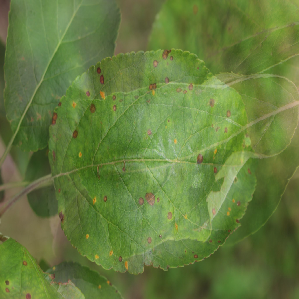
\includegraphics[width=\linewidth]{images/smote_1.png}
\caption{Synthetic image 1}\label{synth1}
\end{subfigure}
\begin{subfigure}[b]{0.49\linewidth}
\centering
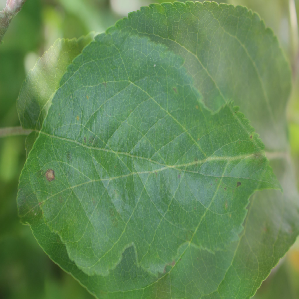
\includegraphics[width=\linewidth]{images/smote_2.png}
\caption{Synthetic image 2}\label{snthy2}
\end{subfigure}\hfill
\end{center}
   \caption{Examples of sythetic samples generated with SMOTE.}
\label{smote}
\end{figure}
Figure \ref{smote} shows some examples of samples generated with SMOTE. 
\subsection{The Combined Model} \label{combined}
The used architecture is a concatenation of a "simple average" ensemble of the presented methods in section \ref{ensemble} and the classfier speciliazed in detection the \textit{Multiple Disease} class presented in section \ref{outlier_detection}. An sketch of the architecture can be seen in figure \ref{architecture}.

\begin{figure}[htb]
\begin{center}
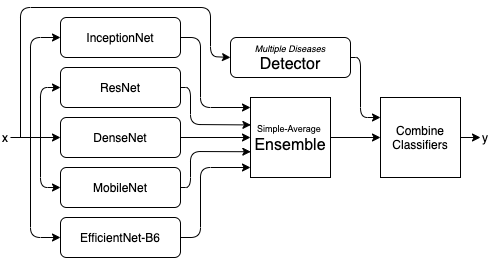
\includegraphics[width=\linewidth]{images/architecture_sketch.png}
\end{center}
   \caption{Sketch of the used architecture for solving the Plant Pathology Challenge.}
\label{architecture}  
\end{figure}

\begin{figure*}[ht]
\begin{center}
    \begin{tabular}{l|S S S r}
      \toprule % <-- Toprule here
       \multirow{2}{*}{\textbf{Classifier}} & \multicolumn{4}{c}{\textbf{F1-Score Per Class}}\\
       & \textbf{Healthy} & \textbf{Multiple Diseases} & \textbf{Rust} & \textbf{Scab}   \\
      \midrule % <-- Midrule here
      \textbf{InceptionNet} & 0.969 & 0.444 & 0.960 & 0.950\\
      \textbf{ResNet} & 0.989 & 0.4 & 0.951 &  0.944 \\
      \textbf{DenseNet} & 0.969 & 0.285 & 0.953 & 0.959\\
      \textbf{MobileNet} & 0.989 & 0.555 & 0.976 & 0.951 \\
       \textbf{EfficientNet-B6} & 0.979 & 0.695 & 0.976 & 0.983 \\
       \textbf{\textit{Multiple Disease} Detector} & 0.888 & 0.991 & 0.888 & 0.888 \\
       \hline
       \textbf{Combined} & 1. & 0.96 & 1. & 0.991 \\
      \bottomrule % <-- Bottomrule here
    \end{tabular}
     \caption{The F1-Score for each neural network used for each class. For the \textit{Multiple Disease} Detector the continuous output is discretized (if the score is $>$0.5 it is classified as \textit{Multiple Diseases} and if it is $\leq$ 0.5 as \textit{Not Multiple Diseases}). Since the \textit{Multiple Disease} Detector only differentiates between these two classes, the score of \textit{Multiple Diseases} is listed under \textit{Multiple Diseases} and \textit{Not Multiple Diseases} under every other class to get an uniform look.}
    \label{tab:f1}
\end{center}
\end{figure*}

%how are they connected
The simple-average Ensembler takes the output of each of the five classifiers and averages them (see section \ref{ensemble}). The output of each classifier is a vector of length four, one value for each class indicating of probable it is that the input is within this class. So the output of the ensembler is logically a vector of length four as well. The \textit{Multiple Disease} detector (section \ref{outlier_detection}) outputs a single number in the range $[0:1]$ indicating how probable it is, that the given input is within the class of \textit{Multiple Diseases}, the higher the more probable. We call this output $prob_{mult}$. So to combine both outputs the output of the \textit{Multiple Disease} detector is extended to the length four as follows: for every class that is not \textit{Multiple Disease} the value will be $1-(prob_{mult})$ and for \textit{Multiple Disease} it is simply the output $prob_{mult}$. This can be formulated as:
\begin{align}
[\frac{1}{p}\sum_{i=1}^{p}(1-\delta)y_i(\mathbf{x})] + \delta \begin{pmatrix} 1-y_{p+1}(\mathbf{x}) \\ y_{p+1}(\mathbf{x}) \\ 1-y_{p+1}(\mathbf{x} \\ 1-y_{p+1}(\mathbf{x}) )\end{pmatrix},
\end{align}
where $y_i(\mathbf{x}) \leq p$ are the classifiers of the ensemble and  $y_{p+1}(\mathbf{x})$ is the \textit{Multiple Disease} detector. $\delta$ is a meta-parameter to indicate how important the \textit{Multiple Diseases} Detector should be. For this work $\delta$ is always set to $0.5$. This setup requires the \textit{Multiple Disease} class to be at index 1.

Each of the classifiers in the ensembler have two additional dense layers appended to the base model, to make the models more flexible. The first has $512$ units and the second $256$ units. Both dense layers have a  ReLU activiation function. In between the two layers is a $30\%$ dropout layer.



Every classifier is loaded with pretrained weights, trained on the ImageNet \cite{deng2009imagenet} dataset. 

All classifiers in the ensemble are trained with the Adam optimizer, a learning rate of $0.001$ and Categorical Cross-Entropy Loss. The \textit{Multiple Disease} detector is trained with Binary Focal Loss \cite{lin2017focal} with $\alpha = 2$ and $\gamma = 0.25$ and the Adam optimizer with a learning rate of $0.001$.

The classifiers of the ensemble have a $4$ unit dense layer with a softmax activiation function as output, to get the desired vector of length four. The \textit{Multiple Disease} detector has a $1$ unit dense layer with a sigmoid activation function as output, to get the desired output in the range of $[0:1]$.

\section{Results}
% What did i find out?

\begin{figure}[htb]
\begin{center}
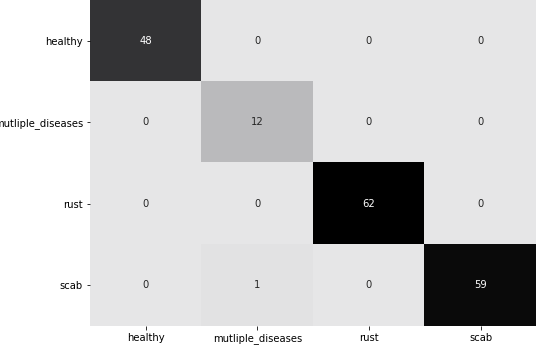
\includegraphics[width=\linewidth]{images/confusion_matrix.png}
\end{center}
   \caption{The confusion matrix on the test dataset (182 images).}
\label{conf_matrix}  
\end{figure}

We trained all models for $200$ epochs and a batch size of $6$. The samples were randomly sampled and augmented like explained in section \ref{augmentation}. All models were tained indenpendently of each other and then combined like described in section \ref{combined}.

Observations have shown that the \textit{Multiple Disease} detector sometimes distorts the result if it is unsure if the sample is within the \textit{Multiple Disease} class. Hence it is only considered if the probability value is above the threshold  $\epsilon = 0.8$. If the probability value is below the threshold $\epsilon$ the output of the detector is not considered (which reduces the model to a simple ensemble classifier).


First of all we look at the performance for each classifier by itself. Table \ref{tab:f1} shows the F1-score for each classifier divided up by class. It is obvious that the \textit{Multiple Diseases} Detector plays a big role in detecting the \textit{Multiple Diseases} class, since all other classifiers are rather confused about this class. The other classes however are detected with very high accuracy. The concept for the architecture is verified to be useful if we look at the table: the standard classifiers deal with the well sampled classes without problem but struggle with the rare \textit{Multiple Diseases} class which is compesated by the \textit{Multiple Diseases} detector. The combined result shows that the composition works. The table also shows that the \textit{Multiple Diseases} detector would need more attetion in an improved version of this architecture since it contains the biggest uncertainties in the whole construct, which also explains why the performance increases if an threshold is introduced (like explained in the last paragraph).

\begin{figure}[htb]
\begin{center}
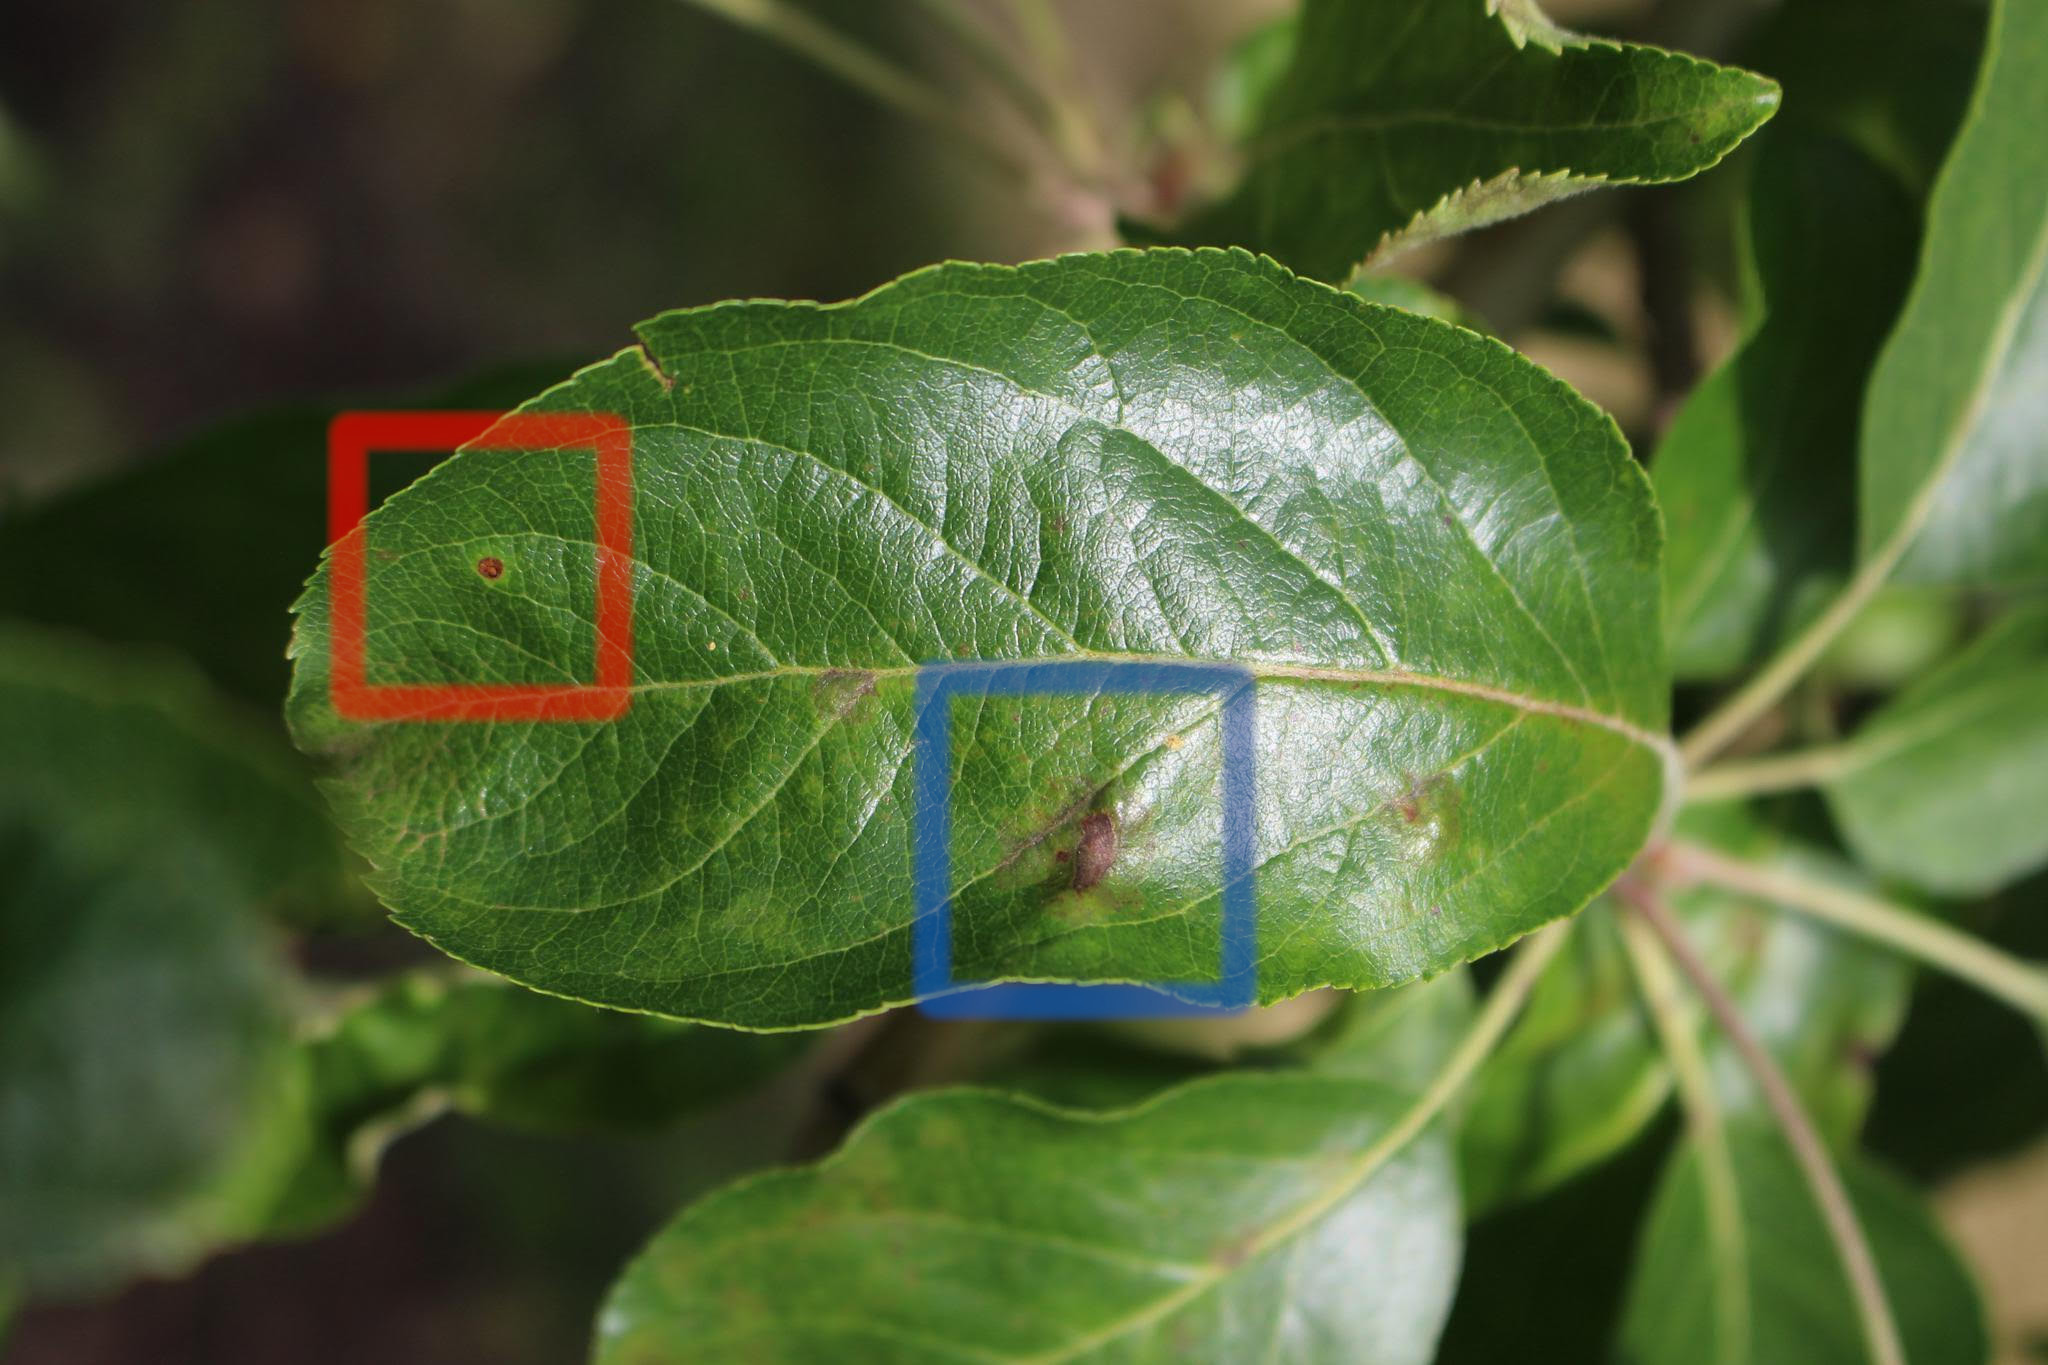
\includegraphics[width=\linewidth]{images/misclassified.jpg}
\end{center}
   \caption{\textit{Rust} image confused as \textit{Multiple Diseases}. Red rectangle shows typical feature for \textit{Rust} class, blue rectangle typical feature for \textit{Scab}.}
\label{miscl}  
\end{figure}

Figure \ref{conf_matrix} shows the resulting confusion matrix on the test data on the combined model. The test data consist of 182 images (48 \textit{Healthy}, 12 \textit{Multiple Diseases}, 62 \textit{Rust} and 60 \textit{Scab}). Only one image was misclassified. This one misclassification confused a \textit{Scab} image as a \textit{Multiple Disease} image. The misclassified image can be seen in figure \ref{miscl}. We assume that this image is falsely classified as \textit{Multiple Disease} because it posses features which could be seen as a mixture of \textit{Rust} (red rectangle) and \textit{Scab} (blue rectangle). 

The trained network architecture achieved a score of $96.6\%$ accuracy on the Kaggle challenge. The accuracy was evaluated on the test dataset of which no labels were given.
\section{Discussion}
% What does it mean?
The score of $96.6\%$ on the public Kaggle leaderboard is not all that great. There are a host of reasons why many scored much better than our solution.

Firstly our image size of $299 \times 299$ is rather small compared to the leading solutions. Leaders of this competition usually used an image sizes at about $700 \times 700$ which enables more fine detection of the features \cite{kaggelLeader1, kaggelLeader2, kaggelLeader3}. Secondly is the simple average ensemble rather naive, a weighted sum would lead to better results since not all classifiers will perform equally good (this would involve to train the weights).   Some competitors pointed out that the data is flawed, so cleaning of the data could have let to less confusion \cite{kaggleData}.

All in all does the architecture seem solid and like a sophisticated approach into dealing with rare classes without suffering classification loss on the other classes.
\section{Conclusion}
In this work we presented an architecture for classifying leafs into multiple classes based solely on image data. We especially tackled the problem of detecting a class which is simultaneously rare and a composition of other existing classes. We did this by training a special classifier which is specialized in detecting whether a sample is of that special rare class. This detector was embedded into a ensemble of classifiers which distinguished between all classes (not only the special rare class). We achieved satisfactory results, if one takes into account that we tried to balance performance and efficiency by scaling the images down highly and only taking network architectures into consideration which are lightweight in terms of computational efficiency.
{\small
\bibliographystyle{ieee_fullname}
\bibliography{bib}
}

\end{document}
